%%%%%%%%%%%%%%%%%%%%%%%%%%%%%%%%%%%%%%%%%
% Masters/Doctoral Thesis 
% LaTeX Template
% Version 2.5 (27/8/17)
%
% This template was downloaded from:
% http://www.LaTeXTemplates.com
%
% Version 2.x major modifications by:
% Vel (vel@latextemplates.com)
%
% This template is based on a template by:
% Steve Gunn (http://users.ecs.soton.ac.uk/srg/softwaretools/document/templates/)
% Sunil Patel (http://www.sunilpatel.co.uk/thesis-template/)
%
% Template license:
% CC BY-NC-SA 3.0 (http://creativecommons.org/licenses/by-nc-sa/3.0/)
%
%%%%%%%%%%%%%%%%%%%%%%%%%%%%%%%%%%%%%%%%%

%----------------------------------------------------------------------------------------
%	PACKAGES AND OTHER DOCUMENT CONFIGURATIONS
%----------------------------------------------------------------------------------------

\documentclass[
11pt, % The default document font size, options: 10pt, 11pt, 12pt
%oneside, % Two side (alternating margins) for binding by default, uncomment to switch to one side
polish, % ngerman for German
singlespacing, % Single line spacing, alternatives: onehalfspacing or doublespacing
%draft, % Uncomment to enable draft mode (no pictures, no links, overfull hboxes indicated)
%nolistspacing, % If the document is onehalfspacing or doublespacing, uncomment this to set spacing in lists to single
%liststotoc, % Uncomment to add the list of figures/tables/etc to the table of contents
%toctotoc, % Uncomment to add the main table of contents to the table of contents
%parskip, % Uncomment to add space between paragraphs
%nohyperref, % Uncomment to not load the hyperref package
headsepline, % Uncomment to get a line under the header
%chapterinoneline, % Uncomment to place the chapter title next to the number on one line
%consistentlayout, % Uncomment to change the layout of the declaration, abstract and acknowledgements pages to match the default layout
]{MastersDoctoralThesis} % The class file specifying the document structure

\usepackage[utf8]{inputenc} % Required for inputting international characters
\usepackage[T1]{fontenc} % Output font encoding for international characters

\usepackage{mathpazo} % Use the Palatino font by default

\usepackage{verbatim}
\usepackage{smartdiagram}

\usepackage{tikz}
\usepackage{pgfplots}
%\usepackage{showframe}
%\usepackage{fancyhdr}
%\usepackage[bottom]{footmisc}
\usepgfplotslibrary{units}
\usepackage{siunitx}


\usepackage[backend=bibtex,style=authoryear,natbib=true]{biblatex} % Use the bibtex backend with the authoryear citation style (which resembles APA)

\addbibresource{example.bib} % The filename of the bibliography

\usepackage[autostyle=true]{csquotes} % Required to generate language-dependent quotes in the bibliography

%----------------------------------------------------------------------------------------
%	MARGIN SETTINGS
%----------------------------------------------------------------------------------------

\geometry{
	paper=a4paper, % Change to letterpaper for US letter
	inner=2.5cm, % Inner margin
	outer=3.8cm, % Outer margin
	bindingoffset=.5cm, % Binding offset
	top=1.5cm, % Top margin
	bottom=1.5cm, % Bottom margin
	%showframe, % Uncomment to show how the type block is set on the page
}

%----------------------------------------------------------------------------------------
%	THESIS INFORMATION
%----------------------------------------------------------------------------------------

\thesistitle{Badanie przetworników piezoelektrycznych} % Your thesis title, this is used in the title and abstract, print it elsewhere with \ttitle
\supervisor{dr. inż. Krzysztof \textsc{Budnik}} % Your supervisor's name, this is used in the title page, print it elsewhere with \supname
\examiner{} % Your examiner's name, this is not currently used anywhere in the template, print it elsewhere with \examname
\degree{Doctor of Philosophy} % Your degree name, this is used in the title page and abstract, print it elsewhere with \degreename
\author{Przemysław \textsc{Sałapata}} % Your name, this is used in the title page and abstract, print it elsewhere with \authorname
\addresses{} % Your address, this is not currently used anywhere in the template, print it elsewhere with \addressname

\subject{Elektrotechnika stosowana} % Your subject area, this is not currently used anywhere in the template, print it elsewhere with \subjectname
\keywords{} % Keywords for your thesis, this is not currently used anywhere in the template, print it elsewhere with \keywordnames
\university{\href{https://www.put.poznan.pl}{Politechnika Poznańska}} % Your university's name and URL, this is used in the title page and abstract, print it elsewhere with \univname
\department{\href{http://department.university.com}{Department or School Name}} % Your department's name and URL, this is used in the title page and abstract, print it elsewhere with \deptname
\group{\href{http://researchgroup.university.com}{Research Group Name}} % Your research group's name and URL, this is used in the title page, print it elsewhere with \groupname
\faculty{\href{http://faculty.university.com}{Faculty Name}} % Your faculty's name and URL, this is used in the title page and abstract, print it elsewhere with \facname

\AtBeginDocument{
\hypersetup{pdftitle=\ttitle} % Set the PDF's title to your title
\hypersetup{pdfauthor=\authorname} % Set the PDF's author to your name
\hypersetup{pdfkeywords=\keywordnames} % Set the PDF's keywords to your keywords
}

\begin{document}

\frontmatter % Use roman page numbering style (i, ii, iii, iv...) for the pre-content pages

\pagestyle{plain} % Default to the plain heading style until the thesis style is called for the body content

%----------------------------------------------------------------------------------------
%	TITLE PAGE
%----------------------------------------------------------------------------------------

\begin{titlepage}
\begin{center}

\vspace*{.06\textheight}
{\scshape\LARGE \univname\par}\vspace{1.5cm} % University name
\textsc{\Large Doctoral Thesis}\\[0.5cm] % Thesis type

\HRule \\[0.4cm] % Horizontal line
{\huge \bfseries \ttitle\par}\vspace{0.4cm} % Thesis title
\HRule \\[1.5cm] % Horizontal line
 
\begin{minipage}[t]{0.4\textwidth}
\begin{flushleft} \large
\emph{Autor:}\\
\href{http://www.johnsmith.com}{\authorname} % Author name - remove the \href bracket to remove the link
\end{flushleft}
\end{minipage}
\begin{minipage}[t]{0.4\textwidth}
\begin{flushright} \large
\emph{Proomotor:} \\
\href{http://www.jamessmith.com}{\supname} % Supervisor name - remove the \href bracket to remove the link  
\end{flushright}
\end{minipage}\\[3cm]
 
\vfill

\large \textit{A thesis submitted in fulfillment of the requirements\\ for the degree of \degreename}\\[0.3cm] % University requirement text
\textit{in the}\\[0.4cm]
\groupname\\\deptname\\[2cm] % Research group name and department name
 
\vfill

{\large \today}\\[4cm] % Date
%\includegraphics{Logo} % University/department logo - uncomment to place it
 
\vfill
\end{center}
\end{titlepage}

%----------------------------------------------------------------------------------------
%	DECLARATION PAGE
%----------------------------------------------------------------------------------------

\begin{declaration}
\addchaptertocentry{\authorshipname} % Add the declaration to the table of contents
\noindent I, \authorname, declare that this thesis titled, \enquote{\ttitle} and the work presented in it are my own. I confirm that:

\begin{itemize} 
\item This work was done wholly or mainly while in candidature for a research degree at this University.
\item Where any part of this thesis has previously been submitted for a degree or any other qualification at this University or any other institution, this has been clearly stated.
\item Where I have consulted the published work of others, this is always clearly attributed.
\item Where I have quoted from the work of others, the source is always given. With the exception of such quotations, this thesis is entirely my own work.
\item I have acknowledged all main sources of help.
\item Where the thesis is based on work done by myself jointly with others, I have made clear exactly what was done by others and what I have contributed myself.\\
\end{itemize}
 
\noindent Signed:\\
\rule[0.5em]{25em}{0.5pt} % This prints a line for the signature
 
\noindent Date:\\
\rule[0.5em]{25em}{0.5pt} % This prints a line to write the date
\end{declaration}

\cleardoublepage

%----------------------------------------------------------------------------------------
%	QUOTATION PAGE
%----------------------------------------------------------------------------------------

\vspace*{0.2\textheight}

\noindent\enquote{\itshape Thanks to my solid academic training, today I can write hundreds of words on virtually any topic without possessing a shred of information, which is how I got a good job in journalism.}\bigbreak

\hfill Dave Barry

%----------------------------------------------------------------------------------------
%	ABSTRACT PAGE
%----------------------------------------------------------------------------------------

\begin{abstract}
\addchaptertocentry{\abstractname} % Add the abstract to the table of contents
The Thesis Abstract is written here (and usually kept to just this page). The page is kept centered vertically so can expand into the blank space above the title too\ldots
\end{abstract}

%----------------------------------------------------------------------------------------
%	ACKNOWLEDGEMENTS
%----------------------------------------------------------------------------------------

\begin{acknowledgements}
\addchaptertocentry{\acknowledgementname} % Add the acknowledgements to the table of contents
The acknowledgments and the people to thank go here, don't forget to include your project advisor\ldots
\end{acknowledgements}

%----------------------------------------------------------------------------------------
%	LIST OF CONTENTS/FIGURES/TABLES PAGES
%----------------------------------------------------------------------------------------

\tableofcontents % Prints the main table of contents

\listoffigures % Prints the list of figures

\listoftables % Prints the list of tables

%----------------------------------------------------------------------------------------
%	ABBREVIATIONS
%----------------------------------------------------------------------------------------

\begin{abbreviations}{ll} % Include a list of abbreviations (a table of two columns)

\textbf{LAH} & \textbf{L}ist \textbf{A}bbreviations \textbf{H}ere\\
\textbf{WSF} & \textbf{W}hat (it) \textbf{S}tands \textbf{F}or\\

\end{abbreviations}

%----------------------------------------------------------------------------------------
%	PHYSICAL CONSTANTS/OTHER DEFINITIONS
%----------------------------------------------------------------------------------------

\begin{constants}{lr@{${}={}$}l} % The list of physical constants is a three column table

% The \SI{}{} command is provided by the siunitx package, see its documentation for instructions on how to use it

Speed of Light & $c_{0}$ & \SI{2.99792458e8}{\meter\per\second} (exact)\\
%Constant Name & $Symbol$ & $Constant Value$ with units\\

\end{constants}

%----------------------------------------------------------------------------------------
%	SYMBOLS
%----------------------------------------------------------------------------------------

\begin{symbols}{lll} % Include a list of Symbols (a three column table)

$a$ & distance & \si{\meter} \\
$P$ & power & \si{\watt} (\si{\joule\per\second}) \\
%Symbol & Name & Unit \\

\addlinespace % Gap to separate the Roman symbols from the Greek

$\omega$ & angular frequency & \si{\radian} \\

\end{symbols}

%----------------------------------------------------------------------------------------
%	DEDICATION
%----------------------------------------------------------------------------------------

\dedicatory{For/Dedicated to/To my\ldots} 

%----------------------------------------------------------------------------------------
%	THESIS CONTENT - CHAPTERS
%----------------------------------------------------------------------------------------

\mainmatter % Begin numeric (1,2,3...) page numbering

\pagestyle{thesis} % Return the page headers back to the "thesis" style

% Include the chapters of the thesis as separate files from the Chapters folder
% Uncomment the lines as you write the chapters

%% Chapter 1

\chapter{Chapter Title Here} % Main chapter title

\label{Chapter1} % For referencing the chapter elsewhere, use \ref{Chapter1} 

%----------------------------------------------------------------------------------------

% Define some commands to keep the formatting separated from the content 
\newcommand{\keyword}[1]{\textbf{#1}}
\newcommand{\tabhead}[1]{\textbf{#1}}
\newcommand{\code}[1]{\texttt{#1}}
\newcommand{\file}[1]{\texttt{\bfseries#1}}
\newcommand{\option}[1]{\texttt{\itshape#1}}


%\chapter{Wprowadzenie}
\label{sec:introduction}

TODO
Do napisania wprowadzenie. Zjawisko piezoelektryczne. Artykuł ma pokazać metodykę projektowania sensorów na konkretnym przykładzie.

\href{http://www.google.com}{przykład linka Google}
%----------------------------------------------------------------------------------------

\section{Welcome and Thank You}
Welcome to this \LaTeX{} Thesis Template, a beautiful and easy to use template for writing a thesis using the \LaTeX{} typesetting system.

If you are writing a thesis (or will be in the future) and its subject is technical or mathematical (though it doesn't have to be), then creating it in \LaTeX{} is highly recommended as a way to make sure you can just get down to the essential writing without having to worry over formatting or wasting time arguing with your word processor. 

\LaTeX{} is easily able to professionally typeset documents that run to hundreds or thousands of pages long. With simple mark-up commands, it automatically sets out the table of contents, margins, page headers and footers and keeps the formatting consistent and beautiful. One of its main strengths is the way it can easily typeset mathematics, even \emph{heavy} mathematics. Even if those equations are the most horribly twisted and most difficult mathematical problems that can only be solved on a super-computer, you can at least count on \LaTeX{} to make them look stunning.

%----------------------------------------------------------------------------------------

\section{Learning \LaTeX{}}

\LaTeX{} is not a \textsc{wysiwyg} (What You See is What You Get) program, unlike word processors such as Microsoft Word or Apple's Pages. Instead, a document written for \LaTeX{} is actually a simple, plain text file that contains \emph{no formatting}. You tell \LaTeX{} how you want the formatting in the finished document by writing in simple commands amongst the text, for example, if I want to use \emph{italic text for emphasis}, I write the \verb|\emph{text}| command and put the text I want in italics in between the curly braces. This means that \LaTeX{} is a \enquote{mark-up} language, very much like HTML.

\subsection{A (not so short) Introduction to \LaTeX{}}

If you are new to \LaTeX{}, there is a very good eBook -- freely available online as a PDF file -- called, \enquote{The Not So Short Introduction to \LaTeX{}}. The book's title is typically shortened to just \emph{lshort}. You can download the latest version (as it is occasionally updated) from here:
\url{http://www.ctan.org/tex-archive/info/lshort/english/lshort.pdf}

It is also available in several other languages. Find yours from the list on this page: \url{http://www.ctan.org/tex-archive/info/lshort/}

It is recommended to take a little time out to learn how to use \LaTeX{} by creating several, small `test' documents, or having a close look at several templates on:\\ 
\url{http://www.LaTeXTemplates.com}\\ 
Making the effort now means you're not stuck learning the system when what you \emph{really} need to be doing is writing your thesis.

\subsection{A Short Math Guide for \LaTeX{}}

If you are writing a technical or mathematical thesis, then you may want to read the document by the AMS (American Mathematical Society) called, \enquote{A Short Math Guide for \LaTeX{}}. It can be found online here:
\url{http://www.ams.org/tex/amslatex.html}
under the \enquote{Additional Documentation} section towards the bottom of the page.

\subsection{Common \LaTeX{} Math Symbols}
There are a multitude of mathematical symbols available for \LaTeX{} and it would take a great effort to learn the commands for them all. The most common ones you are likely to use are shown on this page:
\url{http://www.sunilpatel.co.uk/latex-type/latex-math-symbols/}

You can use this page as a reference or crib sheet, the symbols are rendered as large, high quality images so you can quickly find the \LaTeX{} command for the symbol you need.

\subsection{\LaTeX{} on a Mac}
 
The \LaTeX{} distribution is available for many systems including Windows, Linux and Mac OS X. The package for OS X is called MacTeX and it contains all the applications you need -- bundled together and pre-customized -- for a fully working \LaTeX{} environment and work flow.
 
MacTeX includes a custom dedicated \LaTeX{} editor called TeXShop for writing your `\file{.tex}' files and BibDesk: a program to manage your references and create your bibliography section just as easily as managing songs and creating playlists in iTunes.

%----------------------------------------------------------------------------------------

\section{Getting Started with this Template}

If you are familiar with \LaTeX{}, then you should explore the directory structure of the template and then proceed to place your own information into the \emph{THESIS INFORMATION} block of the \file{main.tex} file. You can then modify the rest of this file to your unique specifications based on your degree/university. Section \ref{FillingFile} on page \pageref{FillingFile} will help you do this. Make sure you also read section \ref{ThesisConventions} about thesis conventions to get the most out of this template.

If you are new to \LaTeX{} it is recommended that you carry on reading through the rest of the information in this document.

Before you begin using this template you should ensure that its style complies with the thesis style guidelines imposed by your institution. In most cases this template style and layout will be suitable. If it is not, it may only require a small change to bring the template in line with your institution's recommendations. These modifications will need to be done on the \file{MastersDoctoralThesis.cls} file.

\subsection{About this Template}

This \LaTeX{} Thesis Template is originally based and created around a \LaTeX{} style file created by Steve R.\ Gunn from the University of Southampton (UK), department of Electronics and Computer Science. You can find his original thesis style file at his site, here:
\url{http://www.ecs.soton.ac.uk/~srg/softwaretools/document/templates/}

Steve's \file{ecsthesis.cls} was then taken by Sunil Patel who modified it by creating a skeleton framework and folder structure to place the thesis files in. The resulting template can be found on Sunil's site here:
\url{http://www.sunilpatel.co.uk/thesis-template}

Sunil's template was made available through \url{http://www.LaTeXTemplates.com} where it was modified many times based on user requests and questions. Version 2.0 and onwards of this template represents a major modification to Sunil's template and is, in fact, hardly recognisable. The work to make version 2.0 possible was carried out by \href{mailto:vel@latextemplates.com}{Vel} and Johannes Böttcher.

%----------------------------------------------------------------------------------------

\section{What this Template Includes}

\subsection{Folders}

This template comes as a single zip file that expands out to several files and folders. The folder names are mostly self-explanatory:

\keyword{Appendices} -- this is the folder where you put the appendices. Each appendix should go into its own separate \file{.tex} file. An example and template are included in the directory.

\keyword{Chapters} -- this is the folder where you put the thesis chapters. A thesis usually has about six chapters, though there is no hard rule on this. Each chapter should go in its own separate \file{.tex} file and they can be split as:
\begin{itemize}
\item Chapter 1: Introduction to the thesis topic
\item Chapter 2: Background information and theory
\item Chapter 3: (Laboratory) experimental setup
\item Chapter 4: Details of experiment 1
\item Chapter 5: Details of experiment 2
\item Chapter 6: Discussion of the experimental results
\item Chapter 7: Conclusion and future directions
\end{itemize}
This chapter layout is specialised for the experimental sciences, your discipline may be different.

\keyword{Figures} -- this folder contains all figures for the thesis. These are the final images that will go into the thesis document.

\subsection{Files}

Included are also several files, most of them are plain text and you can see their contents in a text editor. After initial compilation, you will see that more auxiliary files are created by \LaTeX{} or BibTeX and which you don't need to delete or worry about:

\keyword{example.bib} -- this is an important file that contains all the bibliographic information and references that you will be citing in the thesis for use with BibTeX. You can write it manually, but there are reference manager programs available that will create and manage it for you. Bibliographies in \LaTeX{} are a large subject and you may need to read about BibTeX before starting with this. Many modern reference managers will allow you to export your references in BibTeX format which greatly eases the amount of work you have to do.

\keyword{MastersDoctoralThesis.cls} -- this is an important file. It is the class file that tells \LaTeX{} how to format the thesis. 

\keyword{main.pdf} -- this is your beautifully typeset thesis (in the PDF file format) created by \LaTeX{}. It is supplied in the PDF with the template and after you compile the template you should get an identical version.

\keyword{main.tex} -- this is an important file. This is the file that you tell \LaTeX{} to compile to produce your thesis as a PDF file. It contains the framework and constructs that tell \LaTeX{} how to layout the thesis. It is heavily commented so you can read exactly what each line of code does and why it is there. After you put your own information into the \emph{THESIS INFORMATION} block -- you have now started your thesis!

Files that are \emph{not} included, but are created by \LaTeX{} as auxiliary files include:

\keyword{main.aux} -- this is an auxiliary file generated by \LaTeX{}, if it is deleted \LaTeX{} simply regenerates it when you run the main \file{.tex} file.

\keyword{main.bbl} -- this is an auxiliary file generated by BibTeX, if it is deleted, BibTeX simply regenerates it when you run the \file{main.aux} file. Whereas the \file{.bib} file contains all the references you have, this \file{.bbl} file contains the references you have actually cited in the thesis and is used to build the bibliography section of the thesis.

\keyword{main.blg} -- this is an auxiliary file generated by BibTeX, if it is deleted BibTeX simply regenerates it when you run the main \file{.aux} file.

\keyword{main.lof} -- this is an auxiliary file generated by \LaTeX{}, if it is deleted \LaTeX{} simply regenerates it when you run the main \file{.tex} file. It tells \LaTeX{} how to build the \emph{List of Figures} section.

\keyword{main.log} -- this is an auxiliary file generated by \LaTeX{}, if it is deleted \LaTeX{} simply regenerates it when you run the main \file{.tex} file. It contains messages from \LaTeX{}, if you receive errors and warnings from \LaTeX{}, they will be in this \file{.log} file.

\keyword{main.lot} -- this is an auxiliary file generated by \LaTeX{}, if it is deleted \LaTeX{} simply regenerates it when you run the main \file{.tex} file. It tells \LaTeX{} how to build the \emph{List of Tables} section.

\keyword{main.out} -- this is an auxiliary file generated by \LaTeX{}, if it is deleted \LaTeX{} simply regenerates it when you run the main \file{.tex} file.

So from this long list, only the files with the \file{.bib}, \file{.cls} and \file{.tex} extensions are the most important ones. The other auxiliary files can be ignored or deleted as \LaTeX{} and BibTeX will regenerate them.

%----------------------------------------------------------------------------------------

\section{Filling in Your Information in the \file{main.tex} File}\label{FillingFile}

You will need to personalise the thesis template and make it your own by filling in your own information. This is done by editing the \file{main.tex} file in a text editor or your favourite LaTeX environment.

Open the file and scroll down to the third large block titled \emph{THESIS INFORMATION} where you can see the entries for \emph{University Name}, \emph{Department Name}, etc \ldots

Fill out the information about yourself, your group and institution. You can also insert web links, if you do, make sure you use the full URL, including the \code{http://} for this. If you don't want these to be linked, simply remove the \verb|\href{url}{name}| and only leave the name.

When you have done this, save the file and recompile \code{main.tex}. All the information you filled in should now be in the PDF, complete with web links. You can now begin your thesis proper!

%----------------------------------------------------------------------------------------

\section{The \code{main.tex} File Explained}

The \file{main.tex} file contains the structure of the thesis. There are plenty of written comments that explain what pages, sections and formatting the \LaTeX{} code is creating. Each major document element is divided into commented blocks with titles in all capitals to make it obvious what the following bit of code is doing. Initially there seems to be a lot of \LaTeX{} code, but this is all formatting, and it has all been taken care of so you don't have to do it.

Begin by checking that your information on the title page is correct. For the thesis declaration, your institution may insist on something different than the text given. If this is the case, just replace what you see with what is required in the \emph{DECLARATION PAGE} block.

Then comes a page which contains a funny quote. You can put your own, or quote your favourite scientist, author, person, and so on. Make sure to put the name of the person who you took the quote from.

Following this is the abstract page which summarises your work in a condensed way and can almost be used as a standalone document to describe what you have done. The text you write will cause the heading to move up so don't worry about running out of space.

Next come the acknowledgements. On this page, write about all the people who you wish to thank (not forgetting parents, partners and your advisor/supervisor).

The contents pages, list of figures and tables are all taken care of for you and do not need to be manually created or edited. The next set of pages are more likely to be optional and can be deleted since they are for a more technical thesis: insert a list of abbreviations you have used in the thesis, then a list of the physical constants and numbers you refer to and finally, a list of mathematical symbols used in any formulae. Making the effort to fill these tables means the reader has a one-stop place to refer to instead of searching the internet and references to try and find out what you meant by certain abbreviations or symbols.

The list of symbols is split into the Roman and Greek alphabets. Whereas the abbreviations and symbols ought to be listed in alphabetical order (and this is \emph{not} done automatically for you) the list of physical constants should be grouped into similar themes.

The next page contains a one line dedication. Who will you dedicate your thesis to?

Finally, there is the block where the chapters are included. Uncomment the lines (delete the \code{\%} character) as you write the chapters. Each chapter should be written in its own file and put into the \emph{Chapters} folder and named \file{Chapter1}, \file{Chapter2}, etc\ldots Similarly for the appendices, uncomment the lines as you need them. Each appendix should go into its own file and placed in the \emph{Appendices} folder.

After the preamble, chapters and appendices finally comes the bibliography. The bibliography style (called \option{authoryear}) is used for the bibliography and is a fully featured style that will even include links to where the referenced paper can be found online. Do not underestimate how grateful your reader will be to find that a reference to a paper is just a click away. Of course, this relies on you putting the URL information into the BibTeX file in the first place.

%----------------------------------------------------------------------------------------

\section{Thesis Features and Conventions}\label{ThesisConventions}

To get the best out of this template, there are a few conventions that you may want to follow.

One of the most important (and most difficult) things to keep track of in such a long document as a thesis is consistency. Using certain conventions and ways of doing things (such as using a Todo list) makes the job easier. Of course, all of these are optional and you can adopt your own method.

\subsection{Printing Format}

This thesis template is designed for double sided printing (i.e. content on the front and back of pages) as most theses are printed and bound this way. Switching to one sided printing is as simple as uncommenting the \option{oneside} option of the \code{documentclass} command at the top of the \file{main.tex} file. You may then wish to adjust the margins to suit specifications from your institution.

The headers for the pages contain the page number on the outer side (so it is easy to flick through to the page you want) and the chapter name on the inner side.

The text is set to 11 point by default with single line spacing, again, you can tune the text size and spacing should you want or need to using the options at the very start of \file{main.tex}. The spacing can be changed similarly by replacing the \option{singlespacing} with \option{onehalfspacing} or \option{doublespacing}.

\subsection{Using US Letter Paper}

The paper size used in the template is A4, which is the standard size in Europe. If you are using this thesis template elsewhere and particularly in the United States, then you may have to change the A4 paper size to the US Letter size. This can be done in the margins settings section in \file{main.tex}.

Due to the differences in the paper size, the resulting margins may be different to what you like or require (as it is common for institutions to dictate certain margin sizes). If this is the case, then the margin sizes can be tweaked by modifying the values in the same block as where you set the paper size. Now your document should be set up for US Letter paper size with suitable margins.

\subsection{References}

The \code{biblatex} package is used to format the bibliography and inserts references such as this one \parencite{Reference1}. The options used in the \file{main.tex} file mean that the in-text citations of references are formatted with the author(s) listed with the date of the publication. Multiple references are separated by semicolons (e.g. \parencite{Reference2, Reference1}) and references with more than three authors only show the first author with \emph{et al.} indicating there are more authors (e.g. \parencite{Reference3}). This is done automatically for you. To see how you use references, have a look at the \file{Chapter1.tex} source file. Many reference managers allow you to simply drag the reference into the document as you type.

Scientific references should come \emph{before} the punctuation mark if there is one (such as a comma or period). The same goes for footnotes\footnote{Such as this footnote, here down at the bottom of the page.}. You can change this but the most important thing is to keep the convention consistent throughout the thesis. Footnotes themselves should be full, descriptive sentences (beginning with a capital letter and ending with a full stop). The APA6 states: \enquote{Footnote numbers should be superscripted, [...], following any punctuation mark except a dash.} The Chicago manual of style states: \enquote{A note number should be placed at the end of a sentence or clause. The number follows any punctuation mark except the dash, which it precedes. It follows a closing parenthesis.}

The bibliography is typeset with references listed in alphabetical order by the first author's last name. This is similar to the APA referencing style. To see how \LaTeX{} typesets the bibliography, have a look at the very end of this document (or just click on the reference number links in in-text citations).

\subsubsection{A Note on bibtex}

The bibtex backend used in the template by default does not correctly handle unicode character encoding (i.e. "international" characters). You may see a warning about this in the compilation log and, if your references contain unicode characters, they may not show up correctly or at all. The solution to this is to use the biber backend instead of the outdated bibtex backend. This is done by finding this in \file{main.tex}: \option{backend=bibtex} and changing it to \option{backend=biber}. You will then need to delete all auxiliary BibTeX files and navigate to the template directory in your terminal (command prompt). Once there, simply type \code{biber main} and biber will compile your bibliography. You can then compile \file{main.tex} as normal and your bibliography will be updated. An alternative is to set up your LaTeX editor to compile with biber instead of bibtex, see \href{http://tex.stackexchange.com/questions/154751/biblatex-with-biber-configuring-my-editor-to-avoid-undefined-citations/}{here} for how to do this for various editors.

\subsection{Tables}

Tables are an important way of displaying your results, below is an example table which was generated with this code:

{\small
\begin{verbatim}
\begin{table}
\caption{The effects of treatments X and Y on the four groups studied.}
\label{tab:treatments}
\centering
\begin{tabular}{l l l}
\toprule
\tabhead{Groups} & \tabhead{Treatment X} & \tabhead{Treatment Y} \\
\midrule
1 & 0.2 & 0.8\\
2 & 0.17 & 0.7\\
3 & 0.24 & 0.75\\
4 & 0.68 & 0.3\\
\bottomrule\\
\end{tabular}
\end{table}
\end{verbatim}
}

\begin{table}
\caption{The effects of treatments X and Y on the four groups studied.}
\label{tab:treatments}
\centering
\begin{tabular}{l l l}
\toprule
\tabhead{Groups} & \tabhead{Treatment X} & \tabhead{Treatment Y} \\
\midrule
1 & 0.2 & 0.8\\
2 & 0.17 & 0.7\\
3 & 0.24 & 0.75\\
4 & 0.68 & 0.3\\
\bottomrule\\
\end{tabular}
\end{table}

You can reference tables with \verb|\ref{<label>}| where the label is defined within the table environment. See \file{Chapter1.tex} for an example of the label and citation (e.g. Table~\ref{tab:treatments}).

\subsection{Figures}

There will hopefully be many figures in your thesis (that should be placed in the \emph{Figures} folder). The way to insert figures into your thesis is to use a code template like this:
\begin{verbatim}
\begin{figure}
\centering
%
\includegraphics{Figures/Electron}
\decoRule
\caption[An Electron]{An electron (artist's impression).}
\label{fig:Electron}
\end{figure}
\end{verbatim}
Also look in the source file. Putting this code into the source file produces the picture of the electron that you can see in the figure below.

\begin{figure}[th]
\centering
%
\includegraphics{Figures/Electron}
\decoRule
\caption[An Electron]{An electron (artist's impression).}
\label{fig:Electron}
\end{figure}

Sometimes figures don't always appear where you write them in the source. The placement depends on how much space there is on the page for the figure. Sometimes there is not enough room to fit a figure directly where it should go (in relation to the text) and so \LaTeX{} puts it at the top of the next page. Positioning figures is the job of \LaTeX{} and so you should only worry about making them look good!

Figures usually should have captions just in case you need to refer to them (such as in Figure~\ref{fig:Electron}). The \verb|\caption| command contains two parts, the first part, inside the square brackets is the title that will appear in the \emph{List of Figures}, and so should be short. The second part in the curly brackets should contain the longer and more descriptive caption text.

The \verb|\decoRule| command is optional and simply puts an aesthetic horizontal line below the image. If you do this for one image, do it for all of them.

\LaTeX{} is capable of using images in pdf, jpg and png format.

\subsection{Typesetting mathematics}

If your thesis is going to contain heavy mathematical content, be sure that \LaTeX{} will make it look beautiful, even though it won't be able to solve the equations for you.

The \enquote{Not So Short Introduction to \LaTeX} (available on \href{http://www.ctan.org/tex-archive/info/lshort/english/lshort.pdf}{CTAN}) should tell you everything you need to know for most cases of typesetting mathematics. If you need more information, a much more thorough mathematical guide is available from the AMS called, \enquote{A Short Math Guide to \LaTeX} and can be downloaded from:
\url{ftp://ftp.ams.org/pub/tex/doc/amsmath/short-math-guide.pdf}

There are many different \LaTeX{} symbols to remember, luckily you can find the most common symbols in \href{http://ctan.org/pkg/comprehensive}{The Comprehensive \LaTeX~Symbol List}.

You can write an equation, which is automatically given an equation number by \LaTeX{} like this:
\begin{verbatim}
\begin{equation}
E = mc^{2}
\label{eqn:Einstein}
\end{equation}
\end{verbatim}

This will produce Einstein's famous energy-matter equivalence equation:
\begin{equation}
E = mc^{2}
\label{eqn:Einstein}
\end{equation}

All equations you write (which are not in the middle of paragraph text) are automatically given equation numbers by \LaTeX{}. If you don't want a particular equation numbered, use the unnumbered form:
\begin{verbatim}
\[ a^{2}=4 \]
\end{verbatim}

%----------------------------------------------------------------------------------------

\section{Sectioning and Subsectioning}

You should break your thesis up into nice, bite-sized sections and subsections. \LaTeX{} automatically builds a table of Contents by looking at all the \verb|\chapter{}|, \verb|\section{}|  and \verb|\subsection{}| commands you write in the source.

The Table of Contents should only list the sections to three (3) levels. A \verb|chapter{}| is level zero (0). A \verb|\section{}| is level one (1) and so a \verb|\subsection{}| is level two (2). In your thesis it is likely that you will even use a \verb|subsubsection{}|, which is level three (3). The depth to which the Table of Contents is formatted is set within \file{MastersDoctoralThesis.cls}. If you need this changed, you can do it in \file{main.tex}.

%----------------------------------------------------------------------------------------

\section{In Closing}

You have reached the end of this mini-guide. You can now rename or overwrite this pdf file and begin writing your own \file{Chapter1.tex} and the rest of your thesis. The easy work of setting up the structure and framework has been taken care of for you. It's now your job to fill it out!

Good luck and have lots of fun!

\begin{flushright}
Guide written by ---\\
Sunil Patel: \href{http://www.sunilpatel.co.uk}{www.sunilpatel.co.uk}\\
Vel: \href{http://www.LaTeXTemplates.com}{LaTeXTemplates.com}
\end{flushright}

\chapter{Wprowadzenie}
\label{sec:introduction}

TODO
Do napisania wprowadzenie. Zjawisko piezoelektryczne. Artykuł ma pokazać metodykę projektowania sensorów na konkretnym przykładzie.

\href{http://www.google.com}{przykład linka Google}
\section{Założenia prowadzonych badań}
\label{sec:assumptions}

%\subsection{Wymagania konstrukcyjne}
Źródłem wymuszeń mechanicznych są owalne ciała (bryły sztywne) o masie $m_s=0.03\div1.10 g$ poruszające się torem ruchu przedstawionym na Rys.\ref{fig:route}. Tor wykonany jest ze stalowej rury i w obszarze A (patrz: Rys.\ref{fig:route}) następuje sprężysty kontakt ze ścianą toru. Należy nadmienić, że w obszar A uderza 98\% poruszających się ciał. W odrębnych badaniach ustalono również, że prędkość ciała w momencie kontaktu wynosi $v_s=3.0\div7.0$ $\frac{m}{s}$. Wymuszenia mogą pojawiać się minmalnie w odstępach $T_{smin}=TODO$.

\begin{figure}[htbp]
\centering
\fbox{TUTAJ RYSUNEK TORU RUCHU ZIARNA}%\includegraphics[width=\linewidth]{sample}}
\caption{Zakładany tor lotu ciała fizycznego}
\label{fig:route}
\end{figure}

Założono, że miejscem montażu przetwornika jest obszar A na Rys.\ref{fig:route}, który stanowi okrąg o średnicy $d_p=TODO mm$. Dodatkowo promień ugięcia płaszczyzny A wynosi $R_A=TODOmm$, a kąt padania ciała na tę powierzchnię $\delta_p=135^{\circ}$. 

Tak ściśle i ciekawie przedstawione założenia stały się dobrym punktem wyjścia do szerzej rozumianych badań. Artykuł na naszkicowanym już przykładzie ukazuje zależność odpowiedzi elektrycznej wybranych przetworników PVDF z energią wymuszenia mechanicznego a przede wszystkim kostrukcją (zwaną także geometrią) układu.
\chapter{Metodyka badań}
\label{sec:exp_methods}
Jednym z najważniejszych aspektów badań było zaprojektowanie ich przebiegu. 
 Na Rys.\ref{fig:workflow}. 
 przedstawiono efekt prac nad sposobem realizacji celu eksperymentów. 
 Ważniejszym etapom poświęcono osobny rozdział. Natomiast niewymagającym dłuższego
 komentarza przypisano krótkie wyjaśnienie. 

\begin{figure}[htbp]
\centering
\smartdiagramset{
  set color list={orange, blue,yellow,pink,lime},
  back arrow disabled=true,
  uniform connection color=true,
  description text width=10cm,
  description font = \normalsize,
  module minimum height=1cm,
  descriptive items y sep=2,
  description title width=1cm,
  description title text width=2cm,
  description title font=\scriptsize,
}
% \smartdiagramset{}
\smartdiagram[descriptive diagram]{
{Założenia, Ustalenie założeń konstrukcyjnych czujnika 
(patrz: rozdział \ref{sec:assumptions})},
{Analiza, Separacja założeń mających wpływ na badany układ. },
{Stanowisko, Budowa układu pozwalającego na odizolowanie czynników 
zewnętrznych oraz zapewniającego odpowiednią 
regulację energii zderzenia.(patrz: rozdział \ref{sec:test_stand})},
{Czujniki, Wybór zestawu i rodzaju przetworników do badań.},
{Selekcja czujnika, Badania prowadzące do wyboru optymalnego czujnika.
(patrz: rozdział \ref{sec:sensor_selection})},
{Optymalizacja układu, Eksperymenty prowadzące do optymalizacji przestrzennego 
wyglądu czujnika. Kontrola czujników odrzuconych w kroku poprzednim 
i ewentualny powrót do kroku poprzedniego. 
(patrz: rozdział \ref{sec:construction_optymization})},
{Analiza, Wyznaczenie charakterystyk konstrukcji.
(patrz: rozdział \ref{sec:sensor_characteristic})},
{Analiza, Analiza pozyskanych danych.(patrz: rozdział \ref{sec:conclusion})},
}
\caption{Infografika obrazująca metodykę prowadzonych badań.}
\label{fig:workflow}
\end{figure}

\indent Kluczową rolę w projektowaniu samego przebiegu badań miało przede wszystkim
doprecyzowanie założeń konstrukcyjnych. Pod uwagę wzięto zarówno wejście jak i wyjście
badanego układu. Bardziej doprecyzowane wydaje się być wejście, ponieważ podaje się 
konkretne liczby. Mechanika płynów jest jednak nieprzewidywalnym w $100\%$ zagadnieniem
i dobrze jest przyjąć spory poziom nieufności podczas projektowania. Część dotyczącą
sygnału elektrycznego przedstawiono natomiast ogólnikowo, gdyż układ interpretujący
dopiero zostanie zaprojektowany. Założenia wymagają jedynie zmieszczenia się
parametrów w określonych przedziałach, tak aby zaprojektowanie układu interpretującego
było wykonalne.
\indent Planując metodykę badań skupiono się przede wszystkim na odizolowaniu
środowiska zewnętrznego. Izolacja to nic innego, jak wyodrębnienie sygnału pochodzącego
wyłącznie od przetwornika pobudzonego zderzeniem opisanym w założeniach. Należy tu 
zauważyć, że zbudowane stanowisko pozwoliło osiągnąć szumy na poziomie nie wyższym niż
$40 mV$ i jest to zasługa przede wszystkim wcześniejszego opracowania planu eksperymentów.

\section{Stanowisko badawcze}
\label{sec:test_stand}

Konstrukcję stanowiska badawczego uzależniono od kilku czynników:
%lista punktowana
\begin{itemize}
\item prostota budowy,
\item \textbf{powtarzalność pomiarów},
\item separacja zewnętrznych czynników mogących mieć wpływ na przebieg odpowiedzi elektrycznej,
\item możliwość wymiany modelu przetwornika (patrz: Rys.\ref{fig:test_stand}),
\item łatwa zmiana mocowania przetwornika,
\item możliwość regulacji energii i pędu wymuszenia mechanicznego w zakresie \textbf{$E = 0.24\div14.4$} oraz \textbf{$p = 0.12\div4.8$} obliczonym na podstawie zależności na pęd i energię kinetyczną z fizyki klasycznej \ref{eq:kinetic_energy}.
\end{itemize}

\begin{equation}
E_{s} = \frac{m_{s} \cdot v_{s}^2}{2}
\label{eq:kinetic_energy}
\end{equation}

\begin{equation}
p_{s} = m_{s} \cdot v_{s}
\label{eq:inertia}
\end{equation}
,gdzie: $ m_s$ - masa źródła, $v_s$ - prędkość źródła, $E_s$ - energia kinetyczna źródła, $p_s$ - pęd źródła.

Po podstawieniu danych zawartych w \ref{sec:assumptions} do zależności \ref{eq:kinetic_energy} oraz otrzymano odpowiednio:

%\begin{equation}

$$E_{smin} = \frac{m_{smin} \cdot v_{smin}^2}{2}=\frac{{0.03}\cdot4^2}{2} = {0.24} mJ$$
\\$$p_{smin} = m_{smin} \cdot v_{smin} = {0.03}\cdot 10^{-3} \cdot 4 = {0.12} \cdot 10^{-3}\frac{kg \cdot m}{s^2}$$
\\$$E_{smax} = \frac{m_{smax} \cdot v_{smax}^2}{2}=\frac{0.80\cdot6^2}{2} = 14.4 mJ$$
\\$$p_{smax} = m_{smax} \cdot v_{smax} = 0.80 \cdot 6 = 4.8 \cdot 10^{-3} \frac{kg \cdot m}{s^2}$$

%\end{equation}

\indent %akapit
Biorąc pod uwagę powyższe założenia zdecydowano o zastosowaniu napędu sprężynowego w projektowanym stanowisku. Z tego powodu rozpoczęto pracę od doboru sprężyny. Głównymi kryteriami doboru były wpółczynnik sprężystości sprężyny oraz jej długość. Na podstawie zależności \ref{eq:spring} Wybrano sprężynę o $k=0.17\frac{N}{mm}$ i długości $l=80mm$. Następnie zaprojektowano
%\footnote{Szczegółowy projekt stanowiska dostępny pod \href{http://www.google.com}{adresem}}%TODO
układ przedstawiony na Rys.\ref{fig:test_stand}. Element symulujący źródło impulsu mechanicznego przewidziano wykonać z drewnianej sklejki o masie $m_s = 3.60g$. Na zdjęciu Rys.\ref{fig:test_stand_photo} przedstawiono również realizację wspomnianego stanowiska.

\begin{equation}
E_s = E_p = k \cdot x^2
\label{eq:spring}
\end{equation}
,gdzie: $E_p$ - energia potencjalna sprężystości $k$ - współczynnik sprężystości, $x$ - odkształcenie sprężyny.


\begin{figure}[htbp]
\centering
\fbox{TUTAJ PROJEKT STANOWISKA}%\includegraphics[width=\linewidth]{sample}}
\caption{Projekt stanowiska badawczego.}
\label{fig:test_stand}
\end{figure}

\begin{figure}[htbp]
\centering
%\fbox{
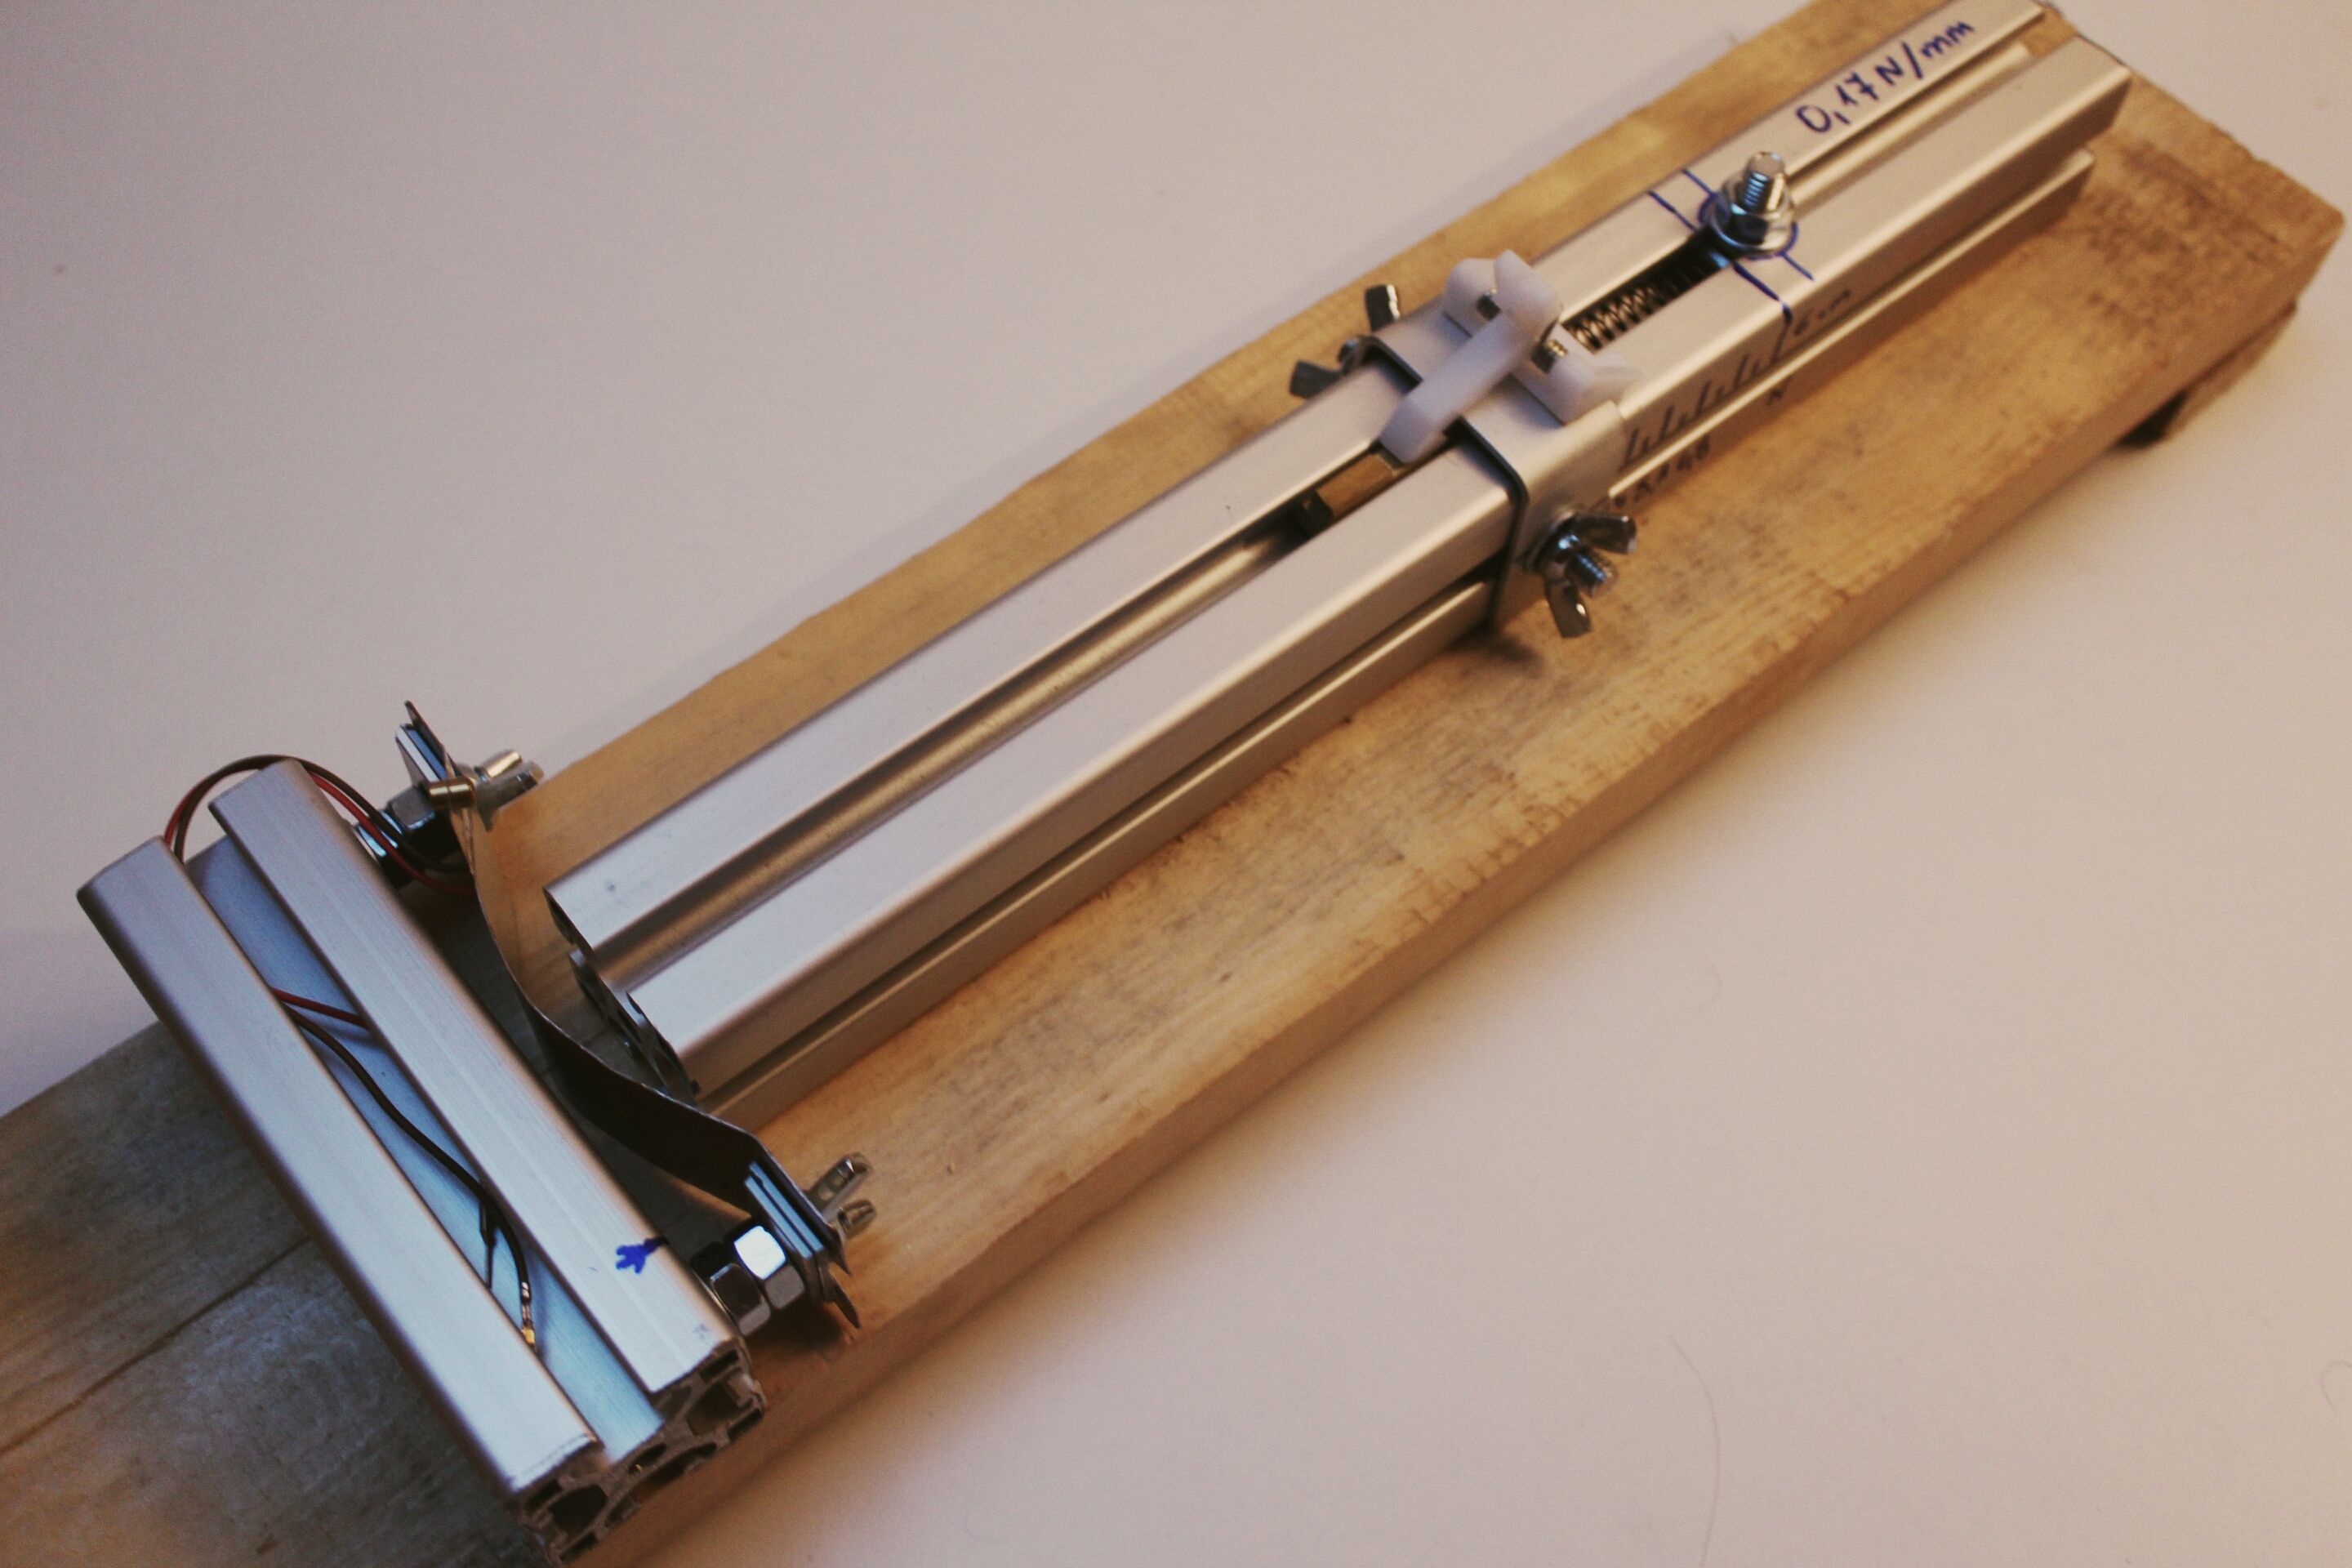
\includegraphics[width=\linewidth]{pictures/lab_stand.jpg}
%}
\caption{Realizacja stanowiska badawczego.}
\label{fig:test_stand_photo}
\end{figure}

Tak skonstruowane stanowisko pozwoliło uzyskać charakterystyki mechaniczne $E(x)$ i $p(x)$ przedstawione na Rys.\ref{fig:mech_char}. Gdyby wziąć pod uwagę możliwość wymiany sprężyny oraz elementu wprawianego w ruch otrzymanoby całą rodzinę charakterystyk, a przez to większą uniwersalność urządzenia.

\pgfplotsset{width=\linewidth,compat=1.3}



\begin{figure}[htbp]
\centering
    \begin{tikzpicture}
%    \pgfplotsset{
%    scale only axis,
%    scaled x ticks=base 10:3,
%    xmin=0, xmax=0.06
%}
      \begin{axis}[
          width=\linewidth, % Scale the plot to \linewidth
          grid=major, % Display a grid
          grid style={dashed,gray!30}, % Set the style
          xlabel=${\delta}x$ , % Set the labels
          ylabel=$E_k$,
          x unit=\si{\milli\metre}, % Set the respective units
          y unit=\si{\milli\joule},
          legend style={at={(0.5,-0.2)},anchor=north}, % Put the legend below the plot
          %x tick label style={rotate=90,anchor=east} % Display labels sideways
        ]
        \addplot[smooth,mark=*,blue] table[x=x,y=E-W,col sep=comma] {pomiary.csv};
        \label{plot_two}
        \addlegendentry{plot 2}
        \end{axis}


        \begin{axis}[
          axis y line*=right,
          axis x line=none,
          width=\linewidth, 
          ylabel=$p$,
          y unit=\si{\k\g\m\per\square\s},
        ] 
        \addlegendimage{/pgfplots/refstyle=plot_one}\addlegendentry{plot 1}
        \addplot[smooth,mark=x,red] table[x=x,y=p,col sep=comma] {pomiary.csv};
        \addlegendentry{plot 3} 
%        \legend{Plot, Plot2}
      \end{axis}
    
%      \begin{axis}[
%          width=\linewidth, % Scale the plot to \linewidth
%          grid=major, % Display a grid
%          grid style={dashed,gray!30}, % Set the style
%          xlabel=${\delta}x$ , % Set the labels
%          ylabel=$E_k$,
%          x unit=\si{\milli\metre}, % Set the respective units
%          y unit=\si{\milli\joule},
%          legend style={at={(0.5,-0.2)},anchor=north}, % Put the legend below the plot
%          %x tick label style={rotate=90,anchor=east} % Display labels sideways
%        ]
%        \addplot table[x=x,y=E-W,col sep=comma] {pomiary.csv};
%        \end{axis}
%        \begin{axis}[
%          axis y line*=right,
%          axis x line=none,
%          width=\linewidth, 
%          ylabel=$p$,
%          %y unit=\si{\k\g\m\per\square\s},
%        ] 
%        \addplot table[x=x,y=p,col sep=comma] {pomiary.csv}; 
%%        \legend{Plot, Plot2}
%      \end{axis}
    \end{tikzpicture}
\caption{Charakterystyka mechaniczna stanowiska badawczego.}
\label{fig:mech_char}
\end{figure}


%sekcja wyboru czujnika piezo
\chapter{Selekcja czujnika}
\label{sec:sensor_selection}

\section{Przegląd rynku piezoelektryków}
\label{sec:piezoelectric_research}

Równolegle z pracami nad stanowiskiem badawczym przeprowadzono przegląd dostępnych
na rynku przetworników piezoelektrycznych. Uwagę skoncentrowano przede wszystkim 
na przetwornikach PVDF
\footnote{Polifluorek winylidenu - 
materiał piezoelektryczny charakteryzujący się elastycznością.}

Do badań wybrano 6 konkretnych produktów (patrz: Rys.\ref{fig:sensors}.):

\begin{enumerate}
\item Czujnik TODO
\item Czujnik TODO
\item Czujnik TODO
\item Czujnik TODO
\item Czujnik TODO
\item Czujnik TODO
\end{enumerate}


\begin{figure}[tbhp]
\centering
\includegraphics[width=\linewidth]{pictures/sensors.jpg}
\caption{Badane przetworniki piezoelektryczne.}
\label{fig:sensors}
\end{figure}

\pagebreak

\section{Wybór optymalnego przetwornika}
\label{sec:optimal_piezoelectric_selection}

Aby dokonać selekcji przetwornika wybrano najprostszy, belkowy układ konstrukcyjny 
(patrz: Rys. \ref{fig:sensor_sel_geometry}). Został on wykonany z fragmentu 
tworzywa sztucznego. Układ oznaczono tak, aby można było ustawić go ponownie 
w tej samej pozycji po wymianie sensora. Sensor przyklejano na taśmę dwustronną 
o grubości ok. $ d = 1.5 mm$ w ustalonym uprzednio miejscu. Na temat
belkowych przetworników piezoelektrycznych można dowiedzieć się więcej 
z pozycji literaturowej \cite{belkowy_sensor}. 

\begin{figure}[tbhp]
\centering
\fbox{TUTAJ RYSUNEK GEOMETRII CZUJNIKA }%\includegraphics[width=\linewidth]{sample}}
\caption{Konstrukcja pozwalająca na selekcję przetwornika piezoelektrycznego.}
\label{fig:sensor_sel_geometry}
\end{figure}

\pagebreak 
W celu uzyskania szerszego spektrum danych dla każdego czujniaka wykonano
poamiary w dwóch wariantach: 
\begin{enumerate}
\item stała podpora na jednym z końców układu przetwornika, drugi koniec swobodny,\nopagebreak
\item stała podpora na jednym z końców układu przetwornika, drugi koniec z 
amortyzatorem z gąbki.
\end{enumerate}

Dla każdego pomiaru przeprowadzono po 10 prób, co pozwoliło zebrać dane zawarte w tabeli
\ref{fig:results_sensor_selection}. Dane zostały wstępnie obrobione, to znaczy zestawiono
je w ujęciu statystycznym.
Parametry, jakie wzięto pod uwagę przy ocenie jakości sygnału, to czas trwania 
( od inicjalizacji do wygaszenia ) oraz wartość napięcia międzyszczytowego oznaczanych 
dalej odpowiednio $t_d$ i $V_{pp}$. Ich porównanie po statystycznej analizie 
przedstawiono na Rys.\ref{fig:sensor_statistic}. Wykres oceny jakości sygnału w skali $0\div5$ 
oznacza subiektywną ocenę poziomu zniekształcenia otrzymanego sygnału. Ocena 0 oznacza mocno
zniekształcony sygnał (patrz: rys. \ref{fig:distorted_signal}) , natomiast 5 sygnał nieodkształcony 
lub odkszktałcony w minimalnym stopniu (patrz: rys. \ref{fig:ideal_signal}). 
Należy nadmienić, że podczas badań zwracano uwagę na sposób przyklejenia przetwornika do plastikowego 
płaskownika tak, aby nie fałszowało to przeprowadzanych pomiarów. 
%TODO Tu przydałby się rozkład widmowy sygnału


\pgfplotstableread[col sep=comma]{selekcja_czujnika.csv}\sensorSelTab


\begin{figure}[htbp]
  \centering
  
\pgfplotsset{compat=1.12}
\begin{tikzpicture}

  \begin{groupplot}[
    group style={
        group name=my fancy plots,
        group size=1 by 3,
        xticklabels at=edge bottom,
        xlabels at = edge bottom,
        vertical sep=25pt
    },
    ybar,
    /pgf/bar width=1,
    ymin=0,
    width=\textwidth,
    height=0.4\textwidth,
    axis x line=bottom,
    enlarge x limits=0.25,
    major x tick style = transparent,
    xtick=data,
    xticklabels from table={\sensorSelTab}{probka},
    xticklabel style={rotate=60, font=\scriptsize},
    yticklabel style={font=\scriptsize},
    xlabel style={at={(-0.1,-0.05)}, font=\scriptsize},
    xlabel={próbka},
    ylabel style={font=\scriptsize},
    title style={at={(0.5,1.0)}, font=\footnotesize}, 
    grid = major,
    table/x expr=\coordindex,
    table/col sep=comma,
]

\nextgroupplot[ylabel={$V_{pp}[V]$},
               ymax=30,
               ytick distance = 10,
               title={Maksymalne napięcie międzyszczytowe},
              ]
\addplot [fill = red] table[y=vpp]{selekcja_czujnika.csv};     

\nextgroupplot[ymode=log,
               ylabel={$t_d[ms]$},
               title={Czas trwania sygnału},
               ]
\addplot [fill = green] table[y=dt]{selekcja_czujnika.csv};;
\nextgroupplot[ymax=5,
               ylabel={$Q[b.j.]$},
               ytick distance = 1,
               title={Ocena jakości sygnału},
               ]
\addplot [fill = blue] table[y=jakość]{selekcja_czujnika.csv};                 
\end{groupplot}

\end{tikzpicture}

\caption{Zestawienie parametrów sygnałów dla poszczególnych czujników na
 podstawie tablicy \ref{fig:results_sensor_selection}.}
\label{fig:sensor_statistic}
\end{figure}


\indent Na podstawie rys.\ref{fig:sensor_statistic} można stwierdzić, że najwyższą wartość
 uzyskanego napięcia $V_{pp}$ otrzymano dla czujnika oznaczonego numerem \textbf{6}.
 Nie gorzej wypadł w tej klasyfikacji przetwornik \textbf{1.1.} Biorąc pod uwagę
 niepewność pomiarową można stwierdzić, że prowadzenie czujnika 6. jest pomijalnie małe.
 Ranking 5 próbek o najlepszych rezultatach przedstawiono dla czytelności w tablicy 
 \ref{fig:sensor_selection_rank_vpp}. 
 \indent Szacuje się, że wyższa wartość $V_{pp}$ będzie bradziej odporna na szumy pochodzące 
 z maszyny, na której sensor byłby umieszczony. Zgodnie z założeniami przeznaczeniem 
 sensora jest przecież licznik impulsów mechanicznych. Z dużym prawdopodobieństwem 
 można uznać, że wyzwalanie licznika następować będzie na jednym ze zboczy pierwszej 
 półfali sygnału (patrz przebieg na rys. \ref{fig:scope_with_silencer}). Nieco inaczej będzie to wyglądać w przypadku sygnału wyprostowanego
 lub nawet stabilizowanego. Takie przekształcenie ułatwi identyfikację wystąpienia 
 wymuszenia. 

 \indent Spoglądając ponownie na wykres $V_{pp}$ na rys. \ref{fig:sensor_statistic}
 można dostrzec pewną ciekawą prawidłowość. Otóż, pomijając czujnik 6., którego sposób
 montażu był nieco inny, wartości napięcia międzyszczytowego dla układów z jedną podporą
 tłumiącą były niższe niż ich odpowiedniki w układach bez drugiej podpory. Wyjaśnieniem
 tego zjawiska jest fakt, iż podpora tłumiąca przecidziała wymuszeniu mechanicznemu i 
 zmniejsza wychylenie belki przetwornika w stosunku do belki wyłącznie z jedną podporą.
 Uzupełnienie informacji w tym temacie zawiera pozycja \cite{belkowy_sensor}.


\begin{table}[h]
  \caption{Ranking optymalizacji pod względem napięcia międzyszczytowego $V_{pp}$}
  \label{fig:sensor_selection_rank_vpp}

  \centering
  \pgfplotstabletypeset[
  col sep = comma,
  columns = {Np,probka,vpp},
  every head row/.style={before row=\toprule,after row=\midrule},
  every last row/.style={after row=\bottomrule},
  display columns/0/.style={column name={Np.}, column type = {r}},
  display columns/1/.style={string type,column name={Próbka}, column type = {l}},
  display columns/2/.style={column name={$V_{pp} [\si{\volt}]$},
  precision=2,fixed zerofill, column type = {r}, fixed},
  skip rows between index={4}{20}
  ]
  {selekcja_czujnika_vpp.csv}
\end{table}
 
\indent Odnosząc się do czasu trwania sygnału jednoznacznie można stwierdzić, 
że im krótszy tym lepszy. Pozwala to uzyskać wyższą częstotliwość wymuszeń mechanicznych 
bez wystąpienia zjawiska aliasingu. Oczywiście detekcja zbyt krótkiego sygnału może być 
problematyczna. Krótkotrwały sygnał wymaga dużej częstotliwości przełączania układu bramkującego.
Przekłąda się to na szybsze zużycie takiego układu jego cenę oraz dokładność zliczania. 
Można np. wyobrazić sobie ukłąd bramkujący, który załącza się powyżej pewnego napięcia
$V_G$, jeżeli utrzymuje się ono powyżej tego poziomu przes czas większy niż czas reakcji 
obwodu bramkującego $t_{dG}$. Czas ten jest związany przede wszystkim z indukcyjnością 
obwodu bramkujacego. Jeśli czas trwania sygnału będzie mniejszy niż  $t_{dG}$, 
impuls nie zostanie wykryty, a więc nie zliczony przez licznik.
Należy pamiętać, że na etapie projektowym montażu przetwornika nie zawsze znana jest energia
wymuszenia mechanicznego. Na pewno jeszcze trudniejsze do okereślenia są straty tejże energii
podczas zderzenia. Powyższe świadczy, że układ przetwornika powininen być odpowiednio
przewymiarowany ( należy przyjąć współczynnik korekcji ), aby uniknąć błędu zliczania.  

\begin{table}[h]
  \caption{Ranking optymalizacji pod względem czasu trwania sygnału $dt$}
  \label{fig:sensor_selection_rank_dt}

  \centering
  \pgfplotstabletypeset[
  col sep = comma,
  columns = {Np,probka,dt},
  sort,
  sort cmp={float <},
  sort key=dt,
  every head row/.style={before row=\toprule,after row=\midrule},
  every last row/.style={after row=\bottomrule},
  display columns/0/.style={column name={Np.}, column type = {r}},
  display columns/1/.style={string type,column name={Próbka}, column type = {l}},
  display columns/2/.style={column name={$dt [\si{\milli\second}]$},
  precision=2,fixed zerofill, column type = {r}, fixed},
  skip rows between index={4}{20}
  ]{selekcja_czujnika_dt.csv}
\end{table}

\indent Przy wyborze przetwornika PVDF o najkorzystniejszych parametrach zdecydowano
się wziąć pod uwagę jeszcze jedną właściwość. Nazwano ją subiektywną oceną jakości 
sygnału, czyli kolokwializując wartość "nieodkształcenia sygnału". Jak wcześniej wspomniano
przyjmuje ona wartośći z przedziału \textbf{$0 \div 5$}, gdzie niższa ocena oznacza
gorzszą jakość sygnału. Dla poszczególnych modeli przetworników, a właściwie próbek sygnału 
sporządzono ranking jakości i dla pierwszych 5 pozycji przedstawiono w tablicy 
\ref{fig:sensor_selection_rank_qa}. Tu przodują czujniki oznaczone \textbf{5}. oraz \textbf{6}., 
ale nie bez znaczenia pozostaje wymieniany coraz częściej numer \textbf{1.1}.
 Pełne statystyki znajdują się w ujęciu graficznym na rys. \ref{fig:sensor_statistic}. 


\begin{table}[h]
  \caption{Ranking optymalizacji pod względem oceny jakości sygnału $Q$}
  \label{fig:sensor_selection_rank_qa}

  \centering
  \pgfplotstabletypeset[
  col sep = comma,
  columns = {Np,probka,jakość},
  sort,
  sort cmp={int >},
  sort key=jakość,
  every head row/.style={before row=\toprule,after row=\midrule},
  every last row/.style={after row=\bottomrule},
  display columns/0/.style={column name={Np.}, column type = {r}},
  display columns/1/.style={string type,column name={Próbka}, column type = {l}},
  display columns/2/.style={column name={$Q [b.j.]$ }, column type = {r}},
  skip rows between index={4}{20}
  ]{selekcja_czujnika_qa.csv}
\end{table}

\section{Odpowiedzi elektryczne przetworników}
\label{sec:signal_description}

\indent Podczas wykonywania pomiarów dokonano interesujących obserwacji, o których warto 
wspomnieć. Otóż zauważono zależności kształtu przebiegu sygnału od poszczególnych 
rozwiązań konstrukcyjnych zastosowanych w modelu przetwornika. Pierwszą zauważona relacja
zachodzi pomiędzy stosowaniem tłumienia drgań ( próbki, które w oznaczeniu zawierają małą 
literę "s" ) a czasem gaśnięcia sygnału $t_d$. Po zastosowaniu tłumika drgań w postaci gąbki $t_d$ 
znacząco się skraca. Jest to wniosek dość oczywisty, jednak 
 warto o tym pamiętać konstruując przetworniki piezoelektryczne. Oprócz tłómików czy 
 filtrów elektrycznych są do dyspozycji również mechaniczne. Dla poparcia przedstawionych
 wniosków należy sięgnąć do danych pomiarowych zawartych w talbicy \ref{fig:results_sensor_selection}
 Tak też w układzie z tłumikiem (patrz: Rys.\ref{fig:scope_with_silencer}) czas wygaszania sgnału 
 wynosi $d_t = 14.40 ms$ i jest krótszy niż w układzie bez tłumika 
 $d_t = 164.00 ms$ (patrz: Rys.\ref{fig:scope_without_silencer}.). 
 Znaczna dysproporcja wystąpiła dla każdego kształtu układu pomiarowego.

\indent Analizując dalej wspomniane próbki pomiarów można również dostrzec, że częstotliwość 
podstawowej harmonicznej sygnału ma bardzo zbliżoną wartość. Nie jest to przypadek. 
Dzieje się tak ponieważ jest to główna harmoniczna drgań własnych konstrukcji przetwornika. 
W tym konkretnym przypadku belki o długości $l = 90 mm$ i jednym punkcie mocowania. 
Projektując przetwornik naleźy zwrócić uwagę, aby odstroić drgania własne konstrukcji 
od drgań wymuszających. W innym przypadku uzyskamy szum informacyjny, dojdzie do tak zwanego
zjawiska aliasingu, czyli nałożenia się następujących kolejno po sobie sygnałów. Idąc dalej 
ma to również wpływ na projektowanie elektronicznego układu przetwornika. W obwodach sygnału 
analogowego spodziewa się właśnie częstotliwości drgań własnych przetwornika. W następnym 
rozdziale \ref{sec:construction_optymization} porusza się również zagadnienie zmiany częstotliwości, 
gdy konstrukcja jest belką o dwóch punktach podparcia. 

\indent Napięcie $V_{pp}$ wykazuje się niezmiennością w odniesieniu do przedstawionych do tej pory zmian 
w konstrukcji. Jednak jest ono zależne od zupełnie innego parametru, od energii ciała M 
tuż przed zderzeniem. Jest ona bezpośrednią przyczyną ugięcia belki z przetwornikiem. 
Energia zderzenia, a dokładniej ta stracona, oraz czas kontaktu z belką stanowią ważne parametry 
dla przebiegu sygnału napięciowego przetwornika. Analizując odpowiedź napięciową jednego z przetworników 
(patrz: rys. \ref{fig:scope_with_silencer})
można zauważyć, że w początkowej fazie pierwszy pik napięciowy ma bezwzględną większą wartość niż następny.
Właściwie oba piki można przybliżyć do gasnącego przebiegu sinusoidalnego. Gdy przeanalizowano kolejne okresy
sygnału, spostrzeżono, że każdakolejna półfala ma coraz mniejszą amplitudę. Jest tak, ponieważ przy kolejnych
fazach sygnału belka traci zgromadzoną energię sprężystości. Między innymi jest ona przekształcana w energię
elektryczną generowaną przez piezoelektryk ( więcej na temeat generatorów piezoelektrycznych można znaleźć w 
\cite{To_Do}). Istotnie. Również w przedziale czasowym $0 \div T$ ($T$ - okres
pierwszej harmonicznej sygnału) energia sprężystości belki jest tracona na generację sygnału elektrycznego.
Co dokładnie dzieje się z przepływem energii? Kiedy rysuje się pierwsza półfala sygnału dochodzi do ugięcia
belki przez ciało M. W szczycie napięcia $u_{p}$, który odpowiada maksymalnemu ugięciu belki następuje
zatrzymanie ciała M i cała energia kinetyczna zgromadzona jest w enegii potencjalnej sprężystości belki.
Następnie belka wraca do pozycji neutralnej i energia potencjalna zamienia się w energię kinetyczną ciała M
oraz belki przetwornika. Dalej belka wychyla się w stronę przeciwną, ale już bez kontaktu z ciałem M. Rysuje się 
druga półfala o niższej amplitudzie i przeciwnym znaku. Gdyby pominąć fakt zamiany energii na energię elektryczną
czynną (obwód pomiarowy nieobciążony) oraz brać pod uwagę sygnał dla konstrukcji bez mechanicznego tłumienia
można z przebiegu sygnału obliczyć energię przekazaną do belkowego przetwornika. Otóż spełniona jest
proporcjonalność ze wzoru \ref{eq:energy_prop}. Jeśli wziąć szczyt pierwszej i drugiej półfali
z rys. \ref{fig:scope_with_silencer}, podstawić do \ref{eq:energy_prop} i podzielić oba równania
stronami uzyskamy stosunek energii potencjalnych w pierwszym i drugim półokresie. Otrzymana
w ten sposób wartość stanowi ułamek energii kinetycznej ciała M przed zderzeniem 
(patrz: rys. \ref{fig:mech_char}) przekazanej skonstruowanemu przetwornikowi piezoelektrycznemu.

  
\begin{equation}
E_{ps} /~ u_{p}^2
\label{eq:energy_prop}
\end{equation}
,gdzie $E_{ps}$ - energia potencjalna sprężystości, $u_{p}$ - napięcie szczytowe.

\indent Kiedy otrzymany stosunek oznaczymy przez $k$ to biorc pod uwagę dane zawarte na
rys. \ref{fig:mech_char} ciało M powinno posiadać po zderzeniu energię wyliczoną według
zależności \ref{eq:energy_after_crash}.


\begin{equation}
E_{kE} = (1-k)\dot E_C
\label{eq:energy_after_crash}
\end{equation}

\indent Do powyższych wniosków wraca się również w rozdziale \ref{sec:construction_optymization}.

\begin{figure}[tbph]
\centering
\includegraphics[width=\linewidth]{pictures/1Acs15dt.jpg}
\caption{Przykładowy przebieg pojedynczego sygnału dla próbki oznaczonej 1.1Acs15dt.}
\label{fig:scope_without_silencer}
\end{figure}

\begin{figure}[tbph]
\centering
\includegraphics[width=\linewidth]{pictures/1Acf15dt.jpg}
\caption{Przykładowy przebieg pojedynczego sygnału dla próbki oznaczonej 1.1Acf15dt.}
\label{fig:scope_with_silencer}
\end{figure}

\chapter{Optymalizacja układu geometrycznego}
\label{sec:construction_optymization}
\begin{figure}[htbp]
\centering
\includegraphics[width=\linewidth]{pictures/uklady_geom.pdf}
\caption{Szkic badanych układów konstrukcyjnych sensorów piezoelektrycznych.}
\label{fig:construct_scetch}
\end{figure}
Niełatwe rozważania na temat kierunku badań dotyczących konstrukcji sensora zaowocowały ustaleniami o konieczności zbadania przetwornika:
\begin{enumerate}
\item belkowego ze względu na możliwość odniesienia się do istniejącej literatury(patrz: A na Rys.\ref{fig:construct_scetch}),
\item o kształcie rury z powodu przeznaczenia konstruowanego przetwornika (patrz: B na Rys.\ref{fig:construct_scetch}),
\end{enumerate}

%\section{Wyznaczenie charakterystyk}
\chapter{Podsumowanie}
\label{sec:conclusion}

\indent Przeprowadzone badania miały na celu ocenę możliwości konstrukcji przetwornika 
do określonego zastosowania w przemyśle. Podstawowym wnioskiem z zaprezentowanej dyskusji
wyników jest pozytywna ocena możliwości zastosowania przetworników PVDF we wspomnianym
projekcie. Jak napisano w rozdziale \ref{sec:sensor_characteristic} wyniki zbliżone do
oczekiwanych uzyskano dla czujnika 1.1. (patrz: rys. \ref{fig:sensors}) w układzie 
konstrukcyjnym B (model rury), mocowany do dówch stałych podpór
 oraz S (patrz: rys. \ref{fig:sensor_sel_geometry}). Równie dobre
resultaty dał czujnik 6. w konfiguracji B, także mocowanej do dwóch stałych podpór.
sam czujnik 6., był natomiast mocowany centralnie do konstrukcji B, pozostawiając 
masę rezonansową swobodną. Dla wszystkich trzech wymienionych konstrukcji możliwe jest
wykonanie odpowiedniego przetwornika. Układ oczywiście poza częścią mechaniczną
wymaga czwórnika w postaci filtra oraz układu bramkującego, jak pokazano to na 
rys. \ref{fig:electrical_scheme}. Wyjście z takiego przetwornika byłoby sygnałem 
prostokątnym o zadanej aplitudzie. Realizowane byłoby to poprzez podłączenie zasilania
do konektora $V_{cc}$. Rozwojowo należeałoby prowadzić te badania właśnie w kierunku
konstrukcji odpowiedniego filtra i obwodu bramkującego. 

\indent Omawiana konstrukcja przetwornika mogłaby mieć zastosowanie w przemyśle na
szerszą skalę do detekcji sygnałów mechanicznych wolno zmiennych, a po pewnych 
modyfikacjach nawet szybkozmiennych. Szczególnie trzeba uwzględnienić sygnały w postaci
udarów mechanicznych.
Jedynym wymaganiem jest kontakt przetwornika z elementem maszyny, w którym udar mółgłby
nastąpić. Przetwornik taki może być przytwierdzany również do pudła rezonatorowego
i detekcja wystąpienia udaru mogłaby następować bez bezpośredniego kontaktu. Jednak 
należałoby wtedy odpowiednio zaprojektować ukłąd elektryczny przetwornika, tak aby nasłuch 
był skupiony, nie tyle na amplitudzie sygnału, co częstotliwości. Takie urządzenia, zwane
analizatorami wibroakustycznymi, ocziwiście istnieją, ale są one zazwyczaj mocno rozbudowane.
Celem powyższych badań jest zdecydowanie prostota i optymalizacja ceny produkcji.






%----------------------------------------------------------------------------------------
%	THESIS CONTENT - APPENDICES
%----------------------------------------------------------------------------------------

\appendix % Cue to tell LaTeX that the following "chapters" are Appendices

% Include the appendices of the thesis as separate files from the Appendices folder
% Uncomment the lines as you write the Appendices

%% Appendix A

\chapter{Frequently Asked Questions} % Main appendix title

\label{AppendixA} % For referencing this appendix elsewhere, use \ref{AppendixA}

\section{How do I change the colors of links?}

The color of links can be changed to your liking using:

{\small\verb!\hypersetup{urlcolor=red}!}, or

{\small\verb!\hypersetup{citecolor=green}!}, or

{\small\verb!\hypersetup{allcolor=blue}!}.

\noindent If you want to completely hide the links, you can use:

{\small\verb!\hypersetup{allcolors=.}!}, or even better: 

{\small\verb!\hypersetup{hidelinks}!}.

\noindent If you want to have obvious links in the PDF but not the printed text, use:

{\small\verb!\hypersetup{colorlinks=false}!}.

%\include{Appendices/AppendixB}
%\include{Appendices/AppendixC}

%----------------------------------------------------------------------------------------
%	BIBLIOGRAPHY
%----------------------------------------------------------------------------------------

\printbibliography[heading=bibintoc]

%----------------------------------------------------------------------------------------

\end{document}  
